\documentclass[12pt]{article}
\usepackage{import}
\usepackage[margin=0.5in]{geometry}
\usepackage{graphics}
\usepackage{xcolor}
\usepackage{bbm}
\usepackage[charter]{mathdesign}


\graphicspath{{images/}}

\import{./}{python_highlights.tex}
\import{./}{polish.tex}
\import{./}{math_preambule.tex}
\import{./}{macros.tex}

\title{
    \huge Podstawy Sterowania Optymalnego - Labolatorium 2\\
    \large Modelowanie układów liniowych przy pomocy zmiennych stanu.
}
\author{Prowadzący: mgr inż. Krzysztof Hałas\\
        Wykonał: Ryszard Napierała}
\date{23 Październik 2021}
\setlength{\parindent}{15pt}

\begin{document}
    \maketitle


    \section{Zadanie 2}
        \begin{enumerate}
            \itemc{W języku Python zaimportować biblioteki \emph{numpy, scipy.signal,
                scipy.integrate.solve\_ivp i matplotlib.pyplot}.}{snippets/lab2/zad2_1.py}
            
            \itemc{Wprowadzić wartości $k_p,T,A,B,C,D$}{snippets/lab2/zad2_2.py}

            \item\textbf{Zapisać system w postaci transmitancji wykorzystując
            przykładowo polecenie\\
            \emph{signal.TransferFunction(num,den)}.}
                \python{snippets/lab2/zad2_3.py}

            \item\textbf{Wyznaczyć odpowiedź skokową układu
            (polecenie \emph{signal.step(sys)}) oraz utworzyć jej
            wykres, przykładowo poleceniem \emph{matplotlib.pyplot}.}
                \python{snippets/lab2/zad2_4.py}
                \outputImg{0.75}{lab2/zad2_4.jpg}
                Czy odpowiedź skokowa odpowiada teoretycznym założeniom?\\
                \emph{Odpowiedź skokowa odpowiada teoretycznym założeniom, jest zgodna z
                oczekiwaniami dla obiektu inercyjnego I-go rzędu.}

            \item\textbf{Zapisać system w postaci fazowych zmiennych stanu wykorzystując polecenie\\
            \emph{signal.StateSpace(A,B,C,D)}. Wyznaczyć i wykreślić odpowiedź skokową układu.}
                \python{snippets/lab2/zad2_5.py}
                \begin{shbox}
                    \centering
                    \textbf{Output:} \\
                    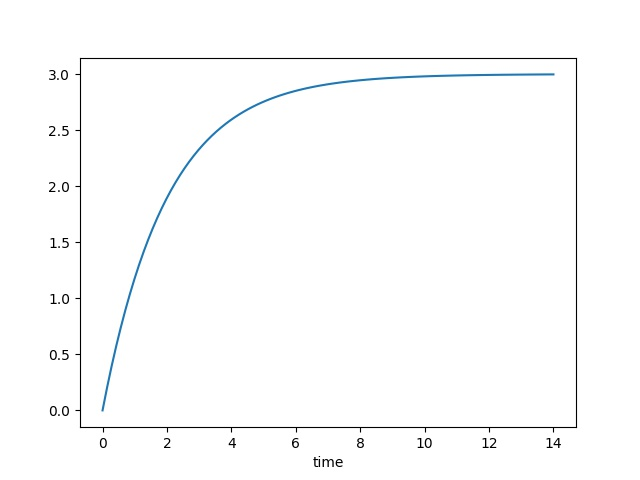
\includegraphics[width=0.75\textwidth]{lab2/zad2_5.jpg}
                \end{shbox}

            \item\textbf{Utworzyć funkcję \emph{model(t,y)} opisującą dynamikę systemu, przyjmującą jako argu-
            menty aktualny czas $(t)$ oraz aktualny stan $(y)$. Przyjąć $u(t) = \mathbbm{1} (t)$.}
                \python{snippets/lab2/zad2_6.py}

            \item\textbf{Utworzyć tablicę wartości czasu $t \in (0, 15)$.}
                \python{snippets/lab2/zad2_7.py}

            \item\textbf{Wyznaczyć rozwiązanie równania dla horyzontu czasowego z poprzedniego podpunktu
            i zerowych warunków początkowych. Wykorzystać komendę solve ivp z odpowiednią
            wartością parametru \emph{t\_eval}. Upewnić się, że model z utworzony w podpunkcie, jest
            zgodny z wymaganiami funkcji \emph{solve\_ivp}.}
                \python{snippets/lab2/zad2_8.py}

            \item\textbf{Wykreślić rozwiązanie równania dla pobudzenia skokiem jednostkowym, wykorzystu-
            jące polecenie \emph{matplotlib.pyplot}. Należy pamiętać o ustawieniu takich samych rozmia-
            rów odpowiednich zmiennych (funkcja \emph{reshape}).}
                \python{snippets/lab2/zad2_9.py}
                \begin{shbox}
                    \centering
                    \textbf{Output:} \\
                    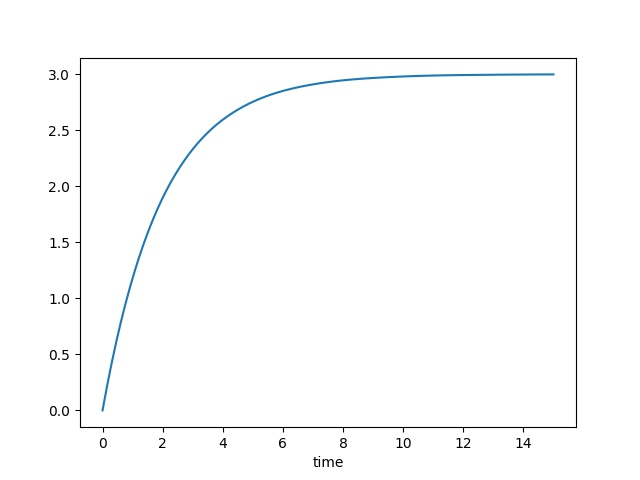
\includegraphics[width=0.75\textwidth]{lab2/zad2_9.jpg}
                \end{shbox}

            \item\textbf{Porównać odpowiedzi skokowe wszystkich trzech reprezentacji
            (systemu opisanemu w postaci transmitancji, w postaci zmiennych stanu oraz
            bezpośredniego rozwiązania równania różniczkowego).}\\
                Odpowiedzi skokowe weszystkich trzech reprezentacji są jednakowe.
        \end{enumerate}

    \section{Zadanie 3}
        \begin{enumerate}
            \item\textbf{W języku Python zamodelować układ dynamiczny przedstawiony na rys. 1 za pomocą
            transmitancji operatorowej oraz wykreślić jego odpowiedzi skokową i impulsową.
            Przyjąć następujące wartości zmiennych $R = 12\Omega$, $L = 1H$ oraz $C = 100\mu F$ .}
                \python{snippets/lab2/zad3_1.py}
                \begin{shbox}
                    \centering
                    \textbf{Output:} \\
                    \begin{tabular}{c}
                        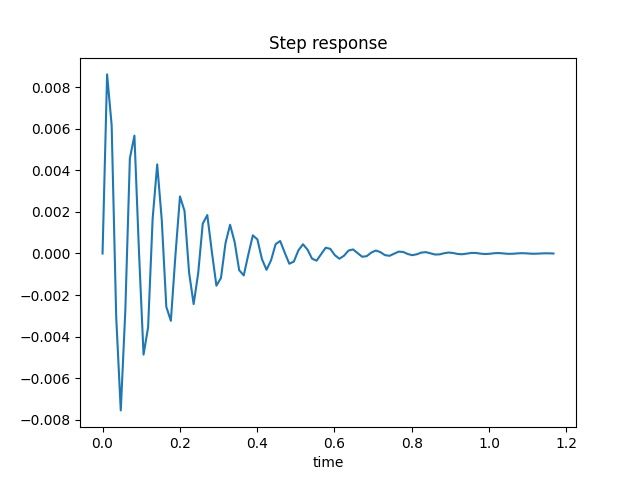
\includegraphics[width=0.45\textwidth]{lab2/zad3_1step.jpg}
                        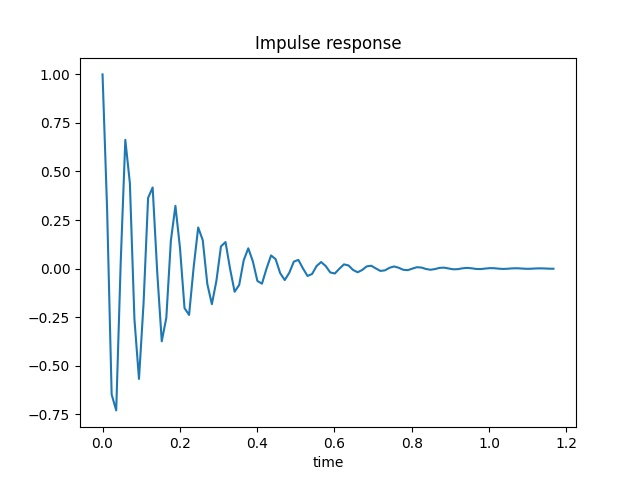
\includegraphics[width=0.45\textwidth]{lab2/zad3_1impulse.jpg}
                    \end{tabular}
                \end{shbox}

            \item\textbf{W języku Python zamodelować ten sam układ przy pomocy zmiennych stanu oraz
            wykreślić jego odpowiedzi czasowe. Porównać z wykresami z poprzedniego podpunktu}
                    \python{snippets/lab2/zad3_2.py}
                    \begin{shbox}
                        \centering
                        \textbf{Output:} \\
                        \begin{tabular}{c}
                            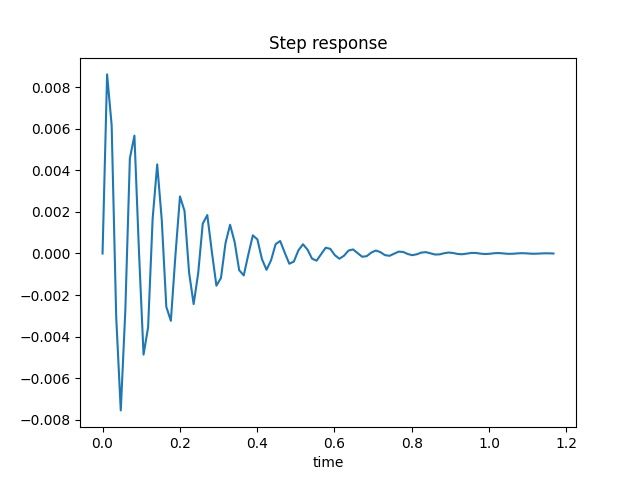
\includegraphics[width=0.45\textwidth]{lab2/zad3_2step.jpg}
                            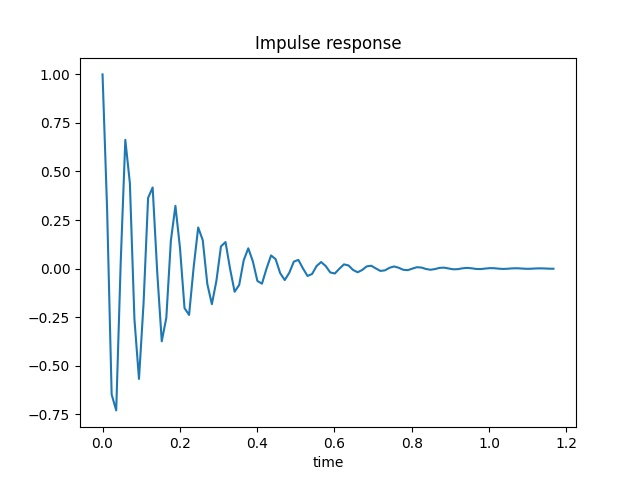
\includegraphics[width=0.45\textwidth]{lab2/zad3_2impulse.jpg}
                        \end{tabular}
                    \end{shbox}
                    Czy wykresy się pokrywają?\\
                    \emph{Wykresy się pokrywają.}

            \item\textbf{Dokonać przekształceń pomiędzy transmitancją a zmiennymi stanu, wykorzystując
            polecenia \emph{tf2ss(num, den)} oraz \emph{ss2tf(A, B, C, D[, input])}.}
                \python{snippets/lab2/zad3_3.py}
                \begin{shbox}
                    \textbf{Output:} \\
                    \lstinputlisting{snippets/lab2/zad3_3out.txt}
                \end{shbox}
                Czy wyprowadzone postaci modeli pokrywają się z tymi wyznaczonymi w Pythonie?\\
                Dlaczego?\\
                \emph{Wyprowadzone postaci modeli pokrywają się z tymi wyznaczonymi w Pythonie.\\
                Jednakże ostatni wspóczynnik w mianowniku \emph{G1 i G2} jest różny,
                co jest spowodowane przybliżeniami liczb zmiennoprzecinkowych, a liczba jest bliska zeru.\\
                \emph{sys1 i sys2} mają zamienione miejscami współczynniki jednakże
                w efekcie końcowym wyniki są równe.\\
                Modele po przekształceniach pokrywają się dlatego że są różnymi reprezentacjami tego samego układu.}

            \item\textbf{Zmienić wartość indukcyjności na $L = 0.15H$. Dokonać przekształceń pomiędzy transmi-
                tancją a zmiennymi stanu.}
                \python{snippets/lab2/zad3_4.py}
                \begin{shbox}
                    \textbf{Output:} \\
                    \lstinputlisting{snippets/lab2/zad3_4out.txt}
                \end{shbox}
                Czy wyprowadzone postaci modeli pokrywają się z tymi wyznaczonymi w Pythonie?\\
                Dlaczego?\\
                \emph{Wyprowadzone postaci modeli pokrywają się z tymi wyznaczonymi w Pythonie.\\
                Modele po przekształceniach pokrywają się dlatego że są różnymi reprezentacjami tego samego układu.}
        \end{enumerate}
    
    \section{Zadanie 4}
        \begin{enumerate}
            \item \textbf{Zakładając następujące zmienne stanu $x_1=\Theta$ i $x_2=\dot{\Theta}$, wejście $u=\tau_m$ oraz wyjście
            $y=x_1$ wyznaczyć równania stanu dla obiektu.}
            \begin{equation*}
                \begin{split}
                    \ddot{\Theta}=\frac{1}{J}\tau_m-\frac{d}{J}\dot{\Theta}\\
                    J=\frac{1}{3}mL^2\\
                    \begin{cases}
                        \dot{x}_1=x_2\\
                        \dot{x}_2=-\frac{d}{J}x_2+\frac{1}{J}u\\
                        y=x_1
                    \end{cases}\\
                    \dot{x}=
                    \begin{bmatrix}
                        \dot{x}_1\\
                        \dot{x}_2
                    \end{bmatrix}=
                    \begin{bmatrix}
                        0& 1\\
                        0& -\frac{d}{J}
                    \end{bmatrix}
                    \begin{bmatrix}
                        x_1\\
                        x_2
                    \end{bmatrix}+
                    \begin{bmatrix}
                        0\\
                        \frac{1}{J}
                    \end{bmatrix}u\\
                    y=
                    \begin{bmatrix}
                        1&0
                    \end{bmatrix}
                    \begin{bmatrix}
                        x_1\\
                        x_2
                    \end{bmatrix}+
                    \begin{bmatrix}
                        0
                    \end{bmatrix}u
                \end{split}
            \end{equation*}
            \python{snippets/lab2/zad4_1.py}

        \item\textbf{Wyznaczyć odpowiedź skokową obiektu wykorzystując polecenie \emph{signal.step(sys2)}.}
            \python{snippets/lab2/zad4_2.py}
            \begin{shbox}
                \centering
                \textbf{Output:} \\
                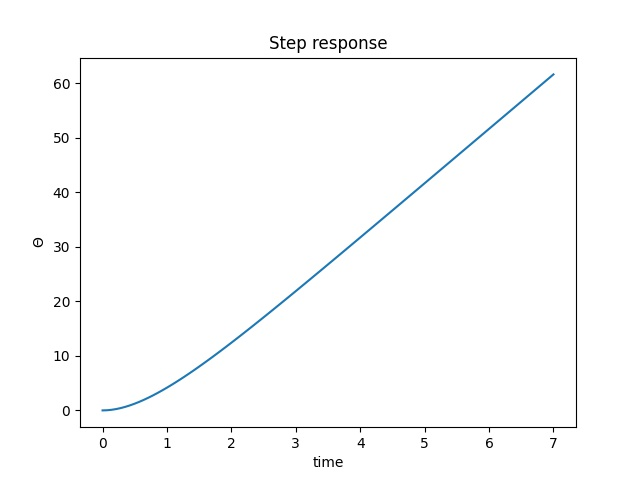
\includegraphics[width=0.75\textwidth]{lab2/zad4_2.jpg}
            \end{shbox}
            Jaki jest charakter odpowiedzi skokowej obiektu?\\
            \emph{Odpowiedź skokowa ma charakter całkujący z inercją.}

        \item\textbf{Wyznaczyć odpowiedzi obiektu dla różnych sygnałów wejściowych (sygnał $\tau_m$ liniowo
        narastający dla wartości początkowej równej $0$, sygnał $\tau_m$ liniowo odpadający dla wartości
        początkowej równej $1$) wykorzystując polecenie \emph{scipy.signal.lsim2}. Do poprawnego
        wykonania zadania konieczna wcześniejsza deklaracja wektorów czasu i zadanego sygnału
        wejściowego.}
            \python{snippets/lab2/zad4_3.py}
            \begin{shbox}
                \centering
                \textbf{Output:} \\
                \begin{tabular}{c}
                    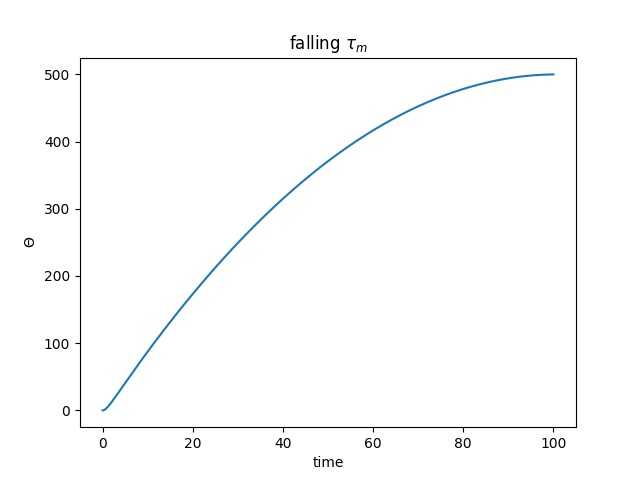
\includegraphics[width=0.45\textwidth]{lab2/zad4_3_falling.jpg}
                    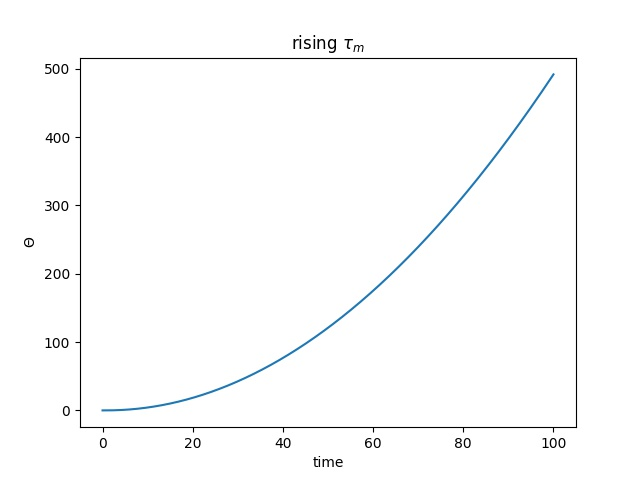
\includegraphics[width=0.45\textwidth]{lab2/zad4_3_rising.jpg}
                \end{tabular}
            \end{shbox}
            Jaki jest charakter odpowiedzi obiektu?\\
            \emph{Odpowiedź ma charakter całkujący z inercją.}

        \item\textbf{Wyznaczyć charakterystykę Bodego dla obiektu wykorzystując
        polecenie \emph{scipy.signal.bode}. Wykreślić charakterystykę w skali logarytmicznej
        wykorzystując polecenie \emph{plt.semilogx}}
            \python{snippets/lab2/zad4_4.py}
            \begin{shbox}
                \centering
                \textbf{Output:} \\
                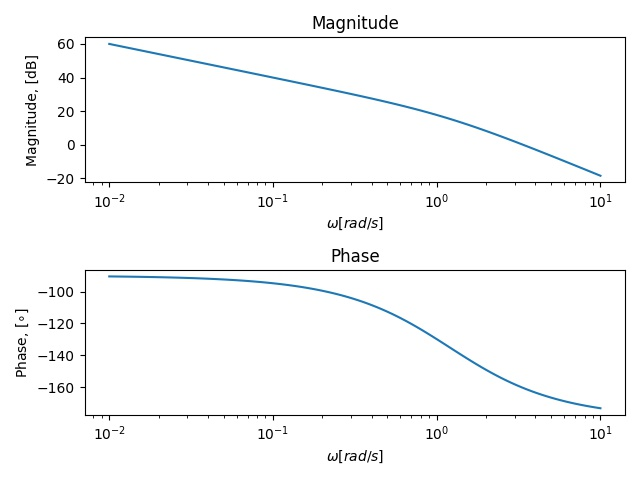
\includegraphics[width=0.75\textwidth]{lab2/zad4_4.jpg}
            \end{shbox}
            Czy wykresy Bodego odpowiadają typowi obiektu?\\
            \emph{Wykresy odpowiadają typowi obiektu.}
        \end{enumerate}
\end{document}